\documentclass[notitlepage]{article}

\usepackage{amssymb}           % dodatni simboli
\usepackage{amsmath}           % eqref, npr.
\usepackage[pdftex]{graphicx}
\usepackage{amsthm}
\usepackage{tikz}
\usepackage[dvipsnames]{xcolor}



\graphicspath{ {./img/} }

\title{Teorija grafov - Zapiski predavanj}
\author{Jakob Drusany}

\newtheorem*{definition}{Definition}
\newtheorem*{theorem}{Theorem}
\newtheorem*{example}{Example}

\begin{document}
\maketitle
\vspace{1cm}
\tableofcontents
\thispagestyle{empty}
\newpage
\pagenumbering{arabic} 
\section{Introduction}
A graph is defined as $G = (V, E)$. $n = |V|$ is the number of vertices, $m = |E|$ is the number of edges.
We also denote them as $V(G), n(G)$, $E(G), m(G)$.
\section{Independence, matching, covers}
\begin{definition}
  The set of vertices $S \subseteq V$ is an \textbf{independent set} if $G(S)$ contains no edges.
  (No two vertices in the independent set are adjacent)
\end{definition}
The independence number $\alpha(G)$ is the size of the maximum independent set.
\begin{definition}
The set of vertices $T \subseteq V$ is a \textbf{vertex cover} if $\forall e \in E$ $T \cap e \neq \emptyset$.
(All edges have at least one endpoint in the vertex cover)
\end{definition}
The vertex cover number $\beta(G)$ is the size of the minimum vertex cover.
\begin{definition}
  A \textbf{matching} is a set of edges $M \subseteq E$ such that $\forall e, f \in M$ $e\neq f$ $e\cap f\neq \emptyset$.
  (No two edges share a vertex)
\end{definition}
The matching number $\alpha'(G)$ is the size of the maximum matching.
\begin{definition}
  An \textbf{edge cover} is a set of edges $C \subseteq E$ such that $\forall v \in V$ $\exists e \in C$ $v \in e$.
  (All vertices are covered by at least one edge from $C$)
\end{definition}
The edge cover number $\beta'(G)$ is the size of the minimum edge cover.
Some graphs have no edge covers, for example graphs with isolated vertices.

\begin{example}
    \begin{figure}[h]
      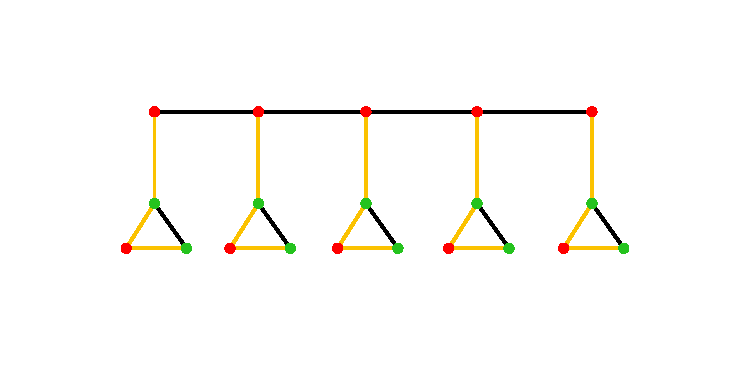
\includegraphics[width=0.8\textwidth]{first_example.pdf}
      \centering
      \caption{$G$ from example}
    \end{figure}

    % text colored red
    \textcolor{BrickRed}{$\alpha(G) = 8$}\\
    \textcolor{blue}{$h(G) = 20$}\\
    \textcolor{OliveGreen}{$\beta(G) = 12$} $\rightarrow$ complement of vertex set\\
    \textcolor{Dandelion}{$\alpha'(G) = 10$} maximum for $\alpha'$ is $\frac{h(G)}{2}$\\
    \textcolor{purple}{$\beta'(G) = 10$}
\end{example}
\newpage
\Large{Observations}
\begin{theorem}
  $\alpha(G) + \beta(G) = |V|$
\end{theorem}
\end{document}